\begin{center}
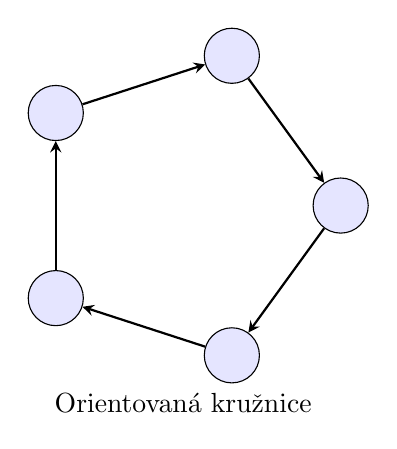
\begin{tikzpicture}[>=stealth, node distance=2cm,
    vnode/.style={circle, draw, minimum size=7mm, inner sep=0pt, fill=blue!10}]
  % Place 5 vertices on a circle without labels
  \foreach \i/\label in {0/A,1/B,2/C,3/D,4/E}{
    \node[vnode] (\label) at ({360/5*\i}:2) {};
  }
  % Draw directed edges forming a cycle
  \foreach \i/\j in {A/B,B/C,C/D,D/E,E/A}{
    \draw[<-, thick] (\i) -- (\j);
  }
  % Centered caption below the diagram
  \node[align=center] at (0,-2.5) {Orientovaná kružnice};
\end{tikzpicture}
\end{center}
